\documentclass[a4paper,11pt,reqno]{amsart}

% --------------------------------------------------------
% Packages
% --------------------------------------------------------
\usepackage[utf8]{inputenc}
\usepackage[foot]{amsaddr}
\usepackage{amsmath,amsfonts,amssymb,amsthm,mathrsfs,bm}
\usepackage[margin=0.95in]{geometry}
\usepackage{color}
\usepackage[dvipsnames]{xcolor}
\usepackage{mathtools,graphicx}
\usepackage{tcolorbox}
\usepackage{listings}
\usepackage{textcomp}
\usepackage{hyperref}

% --------------------------------------------------------
% Custom Colours
% --------------------------------------------------------
\definecolor{CommentGreen}{rgb}{0.0,0.4,0.0}
\definecolor{Background}{rgb}{0.9,1.0,0.85}
\definecolor{lrow}{rgb}{0.914,0.918,0.922}
\definecolor{drow}{rgb}{0.725,0.745,0.769}


% --------------------------------------------------------
% Typesetting Python code
% --------------------------------------------------------
\lstloadlanguages{Python}%
\lstset{
    language=Python, upquote=true, frame=single,
    basicstyle=\small\ttfamily,
    backgroundcolor=\color{yellow!30},
    keywordstyle=[1]\color{NavyBlue}\bfseries,
    keywordstyle=[2]\color{RubineRed},
    keywordstyle=[3]\color{orange!90}\bfseries,
    keywordstyle=[4]\color{Green!90}\bfseries,
    identifierstyle=,
    commentstyle=\usefont{T1}{pcr}{m}{sl}\color{MidnightBlue}\small,
    stringstyle=\color{purple},
    showstringspaces=false, tabsize=4, morekeywords={import,as},
    morekeywords=[2]{args,__init__},
    morekeywords=[3]{@property},
    morekeywords=[4]{self},
    morecomment=[l][\color{blue}]{...},
    numbers=none, firstnumber=1,
    numberstyle=\tiny\color{blue},
    stepnumber=1, xleftmargin=10pt, xrightmargin=10pt
}

\synctex=1

\hypersetup{
    unicode=false, pdftoolbar=true, 
    pdfmenubar=true, pdffitwindow=false, pdfstartview={FitH}, 
    pdftitle={ELE2024 Coursework}, pdfauthor={A. Author},
    pdfsubject={ELE2024 coursework}, pdfcreator={A. Author},
    pdfproducer={ELE2024}, pdfnewwindow=true,
    colorlinks=true, linkcolor=red,
    citecolor=blue, filecolor=magenta, urlcolor=cyan
}

% --------------------------------------------------------
% CUSTOM COMMANDS
% --------------------------------------------------------
\renewcommand{\Re}{\mathbf{re}}
\renewcommand{\Im}{\mathbf{im}}
\newcommand{\R}{\mathbb{R}}
\newcommand{\N}{\mathbb{N}}
\newcommand{\C}{\mathbb{C}}
\newcommand{\lap}{\mathscr{L}}
\newcommand{\dd}{\mathrm{d}}
\newcommand{\smallmat}[1]{\left[ \begin{smallmatrix}#1 \end{smallmatrix} \right]}

% --------------------------------------------------------
% Opening: Title and Author Names
%          Modify this section
% --------------------------------------------------------
\title[ELE2024 Coursework]{LaTeX template for the ELE2024 coursework}

\author[F. Author]{First Author}
\author[A. Someone]{Andreas Someone}
\address[F. Author and A. Someone]{Email addresses: \href{mailto:f.author@qub.ac.uk}%
{f.author@qub.ac.uk} and 
\href{mailto:a.someone.ac.uk}{a.someone@qub.ac.uk}.}
\thanks{Some note goes here.  Version 0.0.1. Last updated:~\today.}



% --------------------------------------------------------
% Beginning of your document
% --------------------------------------------------------
\begin{document}

\maketitle


\section{Part A}
    
    \subsection{Question Q1}\label{sec:q1}
        You may format inline equations using the dollar sign like this $x = 1 = \alpha$ and $y = x^2 - \sqrt{z}$. Equations are like this:
        
        \begin{align}\label{eq:lti_state_update}
            x_{k+1} = A x_k + Bu_k.
        \end{align}
        
        Here is an equation with the Laplace transform
        
        \begin{equation}
            \lap \{e^{at}\} = \frac{1}{s-a},
        \end{equation}
        
        for all complex numbers $s\in\C$ with $\Re(s)>a$. The inverse Laplace transform is denoted like this $\lap^{-1}$.
    
    \subsection{Question Q2}
        Refer to other sections as Section~\ref{sec:q1}. An example of a numbered list
        \begin{enumerate}
            \item first item,
            \item second item.
        \end{enumerate}
        Links are \href{https://google.com}{like this}. We also have \textbf{boldface}, \textit{italics},
        \emph{emphasised}, \texttt{truetype}, \textsc{Small Caps} and so on.
    
    \subsection{More math} Denote the real numbers as $\R$ and the complex numbers as $\C$. Example of a limit:
    
        \begin{equation}
            z = \lim_{s\to0^+}\frac{s+1}{s^3+s^2-5s+9}.
        \end{equation}
        
        Another example
        \begin{equation}
            \lim_{s\to\infty} \frac{s+1}{s^3+s^2-5s+9}.
        \end{equation}
        
        Example of an integral
        \begin{equation}
            \int_0^\infty e^{-s\tau}f(\tau)\dd\tau.
        \end{equation}
        
        Three aligned equations
        \begin{align}
            a =& 1,
            \\
            b =& 2,
            \\
            c =& 3.
        \end{align}
        
        Two aligned equations without equation numbers
        \begin{align*}
            a =& 1,
            \\
            b =& 2.
        \end{align*}
        
        Mathematical derivations aligned at the ``='' sign:
        \begin{align}
            \frac{1}{2+3j} {}={}& \frac{2-3j}{(2+3j)(2-3j)}
            \notag\\
            {}={}& \frac{2-3j}{2^2 + 3^2}
            \notag\\
            {}={}& \frac{2-3j}{13}
            \notag\\
            {}={}&\frac{2}{13} - j\frac{3}{13}.
        \end{align}
        
        More mathematical derivations:
        \begin{align*}
            & as + 4 + 2s = b + (8+a)s
            \\
            \Leftrightarrow{}& (a+2)s + 4 = b + (8+a)s
            \\
            \Leftrightarrow{}& (a+2)s - (8+a)s = b - 4.
        \end{align*}
        
        Boldface math: $\bm{x}$. Vectors:
        \begin{equation}
            \bm{x} = 
            \begin{bmatrix}
                x_1
                \\
                x_2
                \\
                x_3
            \end{bmatrix}.
        \end{equation}
        
        Another example: According to Taylor's Theorem:
        \begin{equation}
            \phi(x) \approx \phi(x_0) + \phi'(x_0)(x-x_0).
        \end{equation}
        
        Partial derivatives:
        \begin{equation}
            \label{eq:partial_derivatives}
            \frac{\partial f(x, y)}{\partial x} = x^2\cos(xy).
        \end{equation}
        
        \begin{tcolorbox}[title={Common typesetting mistakes}]
            \textbf{Important Note:} 
            \begin{itemize}
                \item Write $\cos x$, not $cos x$.
                \item Write $\sin x$, $\log x$, etc --- not $sin x$, $log x$ and so on.
                \item Write $\lim_{s\to 0^+} sF(s)$, not $lim_{s\to 0^+} sF(s)$.
                \item Write $F(s)$, not $F(S)$. 
                \item Write $xy$, or $x\dot y$, but not $x*y$ --- that would be the \textit{convolution} of     $x$ with $y$, not their product, so
                    \begin{equation}
                        2 * 3 = 3t^2.
                    \end{equation}
                \item To denote a variable with a subscript, write $x_1$, not $x1$.
                \item For superscripts, write $x^2$, not $x2$.
                \item Denote a variable by $x$, not x. 
                \item Double quotes are ``like this'', not "like this".
                \item Reference equations using: Equation \eqref{eq:partial_derivatives}; not Equation \ref{eq:partial_derivatives} and not Equation (12).
            \end{itemize}
        \end{tcolorbox}
        
        
        
        % You can write comments like this
        \begin{figure}
            \centering
            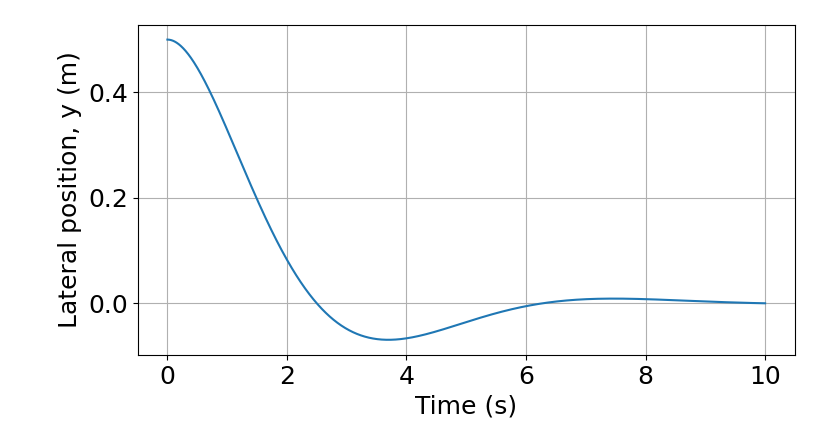
\includegraphics[width=0.65\linewidth]{figures/lateral_position}
            \caption{You may of course include figures in your document. Make sure your figures have legible axis labels. Figures of about this size are perfectly legible.}
        \end{figure}



\end{document}
